\subsection{Fremdrift}

Bilens fremdrift forårsages af motoren samt tilhørende elektronik, hvilket er beskrevet på figur \ref{fig:ibd_fremdrift}. Det skal igen noteres at forsyningen til H-broen ikke er på diagrammet, men findes på figur \ref{fig:ibd_bil_forsyning}. Motoren trækker altså ikke sin strøm fra signalet motorCtrl. 

\begin{figure}[h]
\centering
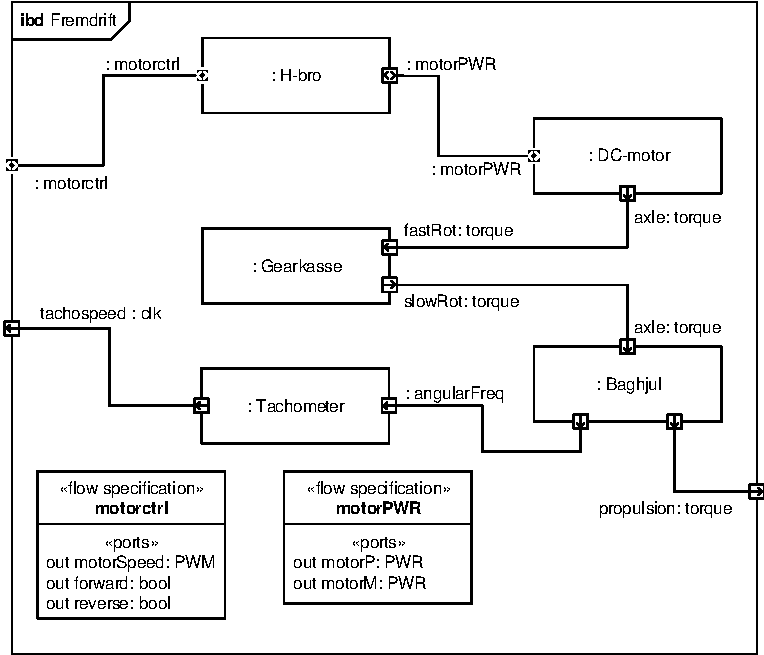
\includegraphics[scale=1]{../fig/diagrammer/bil/ibd_fremdrift.pdf}
\caption{IBD for blokken fremdrift}
\label{fig:ibd_fremdrift}
\end{figure}

\clearpage

\subsubsection{Signalbeskrivelse for fremdrift}

\begin{table}[h]
	\centering
	\begin{tabularx}{\textwidth}{|l|X|X|X|} \hline
	\textbf{Signal (navn: type)} & \textbf{Funktion} & \textbf{Tolerancer} & \textbf{Kommentarer} \\ \hline
motorSpeed: PWM
	& Et PWM signal der bestemmer motorhastigheden. 
	& Frekvens: 30kHz +/- 1kHz 0-5V +/- 0.2V
 	& Logisk signal: \newline
		Lav = 0V +/- 0.2V \newline
		Høj = 5V +/- 0.2V
	\\ \hline

forward: bool
	& Kontrolsignal til H-bro.
	& 0-5V $\pm$ 0.2V
	& Lav = 0V +/- 0.2V  ’idle’ \newline
		Høj =  5V +/- 0.2V  ’frem’
	\\ \hline
	
reverse: bool
	& Kontrolsignal til H-bro.
	& 0-5V $\pm$ 0.2V
	& Lav = 0V +/- 0.2V ’idle’ \newline
		Høj =  5V +/- 0.2V  ’tilbage’
	\\ \hline
	
motorP: PWR
	& Et PWM med frekvens som motorSpeed, dog med mulighed for højere effekt. 			Dette signal forsyner motoren.
	& Frekvens: 30kHz +/- 1kHz 0-7,2V +/- 0.5V

 	& Logisk signal: \newline
		Lav = 0V +/- 0.5V \newline 
		Høj = 7,2V +/- 0.5V
	\\ \hline

motorM: PWR
	& Reference til motorP.
	& 0V $\pm$ 0.5V
	& ~
	\\ \hline
	
fastRot: torque
	& Kraft der overføres fra motor til gearkasse via drivaksel.
	& - 
	& ~
	\\ \hline
	
slowRot: torque
	& Kraft der overføres fra gearkasse til baghjul via drivaksel.
	& - 
	& ~
	\\ \hline
	
: angularFreq
	& Hjulenes omdrejningshastighed.
	& - 
	& ~
	\\ \hline
	
tachoSpeed: freq
	& Digitalt signal med varierende frekvens afhængig af baghjulenes 					omdrejningshastighed.
	& - 
	& Vejledende: \newline
		64Hz = 10Km/t \newline
		Logisk signal: \newline
		Lav = 0V +/- 0.2V \newline
		Høj = 5V +/- 0.2V

	\\ \hline
	
Propulsion: torque
	& Baghjulenes torque til underlaget.
	& - 
	& ~
	\\ \hline
	\end{tabularx}
\end{table}